\section{Phénoménologie des bosons de Higgs du MSSM}\label{chapter-MS-MSSM-section-pheno_Higgs_MSSM}
Pour concevoir une analyse de physique des particules à même de tester le MSSM, il faut dans un premier temps déterminer la manifestation du MSSM à observer.
Comme cela a été développé dans la section précédente, le MSSM implique l'existence de quatre bosons de Higgs supplémentaires, en particulier deux nouveaux bosons de Higgs neutres, \Higgs\ et \HiggsA.
Si de tels bosons existent, un signal leur correspondant doit pouvoir être observé.
\par Au premier ordre, les masses des bosons de Higgs s'expriment en fonction de deux paramètres uniquement, $m_{\HiggsA}$ et $\tan\beta$.
Les couplages des trois bosons de Higgs neutres du MSSM aux autres particules, par rapport aux couplages du boson de Higgs du modèle standard, sont présentés dans le tableau~\ref{tab-Higgs_couplings_2HDM} en fonction de $\alpha$ et $\beta$.
Or, $\alpha$ et $\beta$ sont reliés par les équations~\eqref{eq-Higgs_mixing_angle_MSSM}, donnant
\begin{equation}
\tan 2\alpha = \frac{m_{\HiggsA}^2+m_{\Zboson}^2}{m_{\HiggsA}^2-m_{\Zboson}^2} \tan 2\beta
\mend
\label{eq-Higgs_mixing_angle_MSSM_tan}
\end{equation}
\par Les observations expérimentales semblent favoriser $m_{\HiggsA}\gg m_{\Zboson}$~\cite{ATLAS-CMS-Higgs_combined_1,ATLAS-CMS-Higgs_combined_2,CMS-MSSM-HTT_2014}.
Dans ce cas, \Higgs\ et \HiggsA\ sont de masses similaires et \higgs\ doit jouer le rôle du boson de Higgs du modèle standard observé expérimentalement en 2012~\cite{ATLAS_Higgs_discovery,CMS_Higgs_discovery,CMS_Higgs_discovery_2013}.
Cette situation correspond à la limite découplée, dans laquelle
\begin{equation}
\lim_{m_{\HiggsA}\gg m_{\Zboson}} \tan 2\alpha = \tan 2\beta
\end{equation}
d'après~\eqref{eq-Higgs_mixing_angle_MSSM_tan}.
Alors, dans la limite découplée, $\alpha \sim \beta$ ou $\alpha\sim\beta\pm\frac{\pi}{2}$.
Or, $\beta\geq0$ et $\alpha\leq0$ et $\tan\beta$ est contraint par~\cite{Ridolfi-SUSY}
\begin{equation}
1 < \tan\beta \lesssim \frac{m_{\quarkt}}{m_{\quarkb}} \simeq \num{42} \mend
\end{equation}
Il ne reste donc plus que la possibilité $\alpha\sim\beta-\frac{\pi}{2}$.
Dans la limite découplée, les couplages du tableau~\ref{tab-Higgs_couplings_2HDM} deviennent alors ceux du tableau~\ref{tab-Higgs_couplings_MSSM_decoupling}.
\begin{table}[h]
\centering
\begin{tabular}{rccc}
\toprule
Couplage avec & \higgs & \Higgs & \HiggsA \\
\midrule
Bosons vecteurs & $\sim1$ & $\sim0$ & $0$\\
Fermions hauts & $\sim1$ & $\sim-\cot\beta$ & $\cot\beta$ \\
Fermions bas & $\sim1$ & $\sim\tan\beta$ & $\tan\beta$ \\
\bottomrule
\end{tabular}
\caption[Couplages des bosons de Higgs neutres dans la limite découplée.]{Couplages des bosons de Higgs neutres dans la limite découplée du MSSM par rapport aux couplages du boson de Higgs du modèle standard.}
\label{tab-Higgs_couplings_MSSM_decoupling}
\end{table}
\par Les couplages ainsi obtenus dans le tableau~\ref{tab-Higgs_couplings_MSSM_decoupling} présentent trois caractéristiques d'intérêt:
\begin{itemize}
\item le boson de Higgs le plus léger, \higgs, se comporte comme le boson de Higgs du modèle standard, ce qui le rend tout à fait cohérent avec les observations actuelles;
\item les bosons de Higgs neutres massifs \Higgs\ et \HiggsA\ présentent peu voire aucun couplage aux bosons vecteurs, par exemple la désintégration $\HiggsA\to\Zboson\Zboson$ est impossible mais $\HiggsA\to\Zboson\higgs$ est possible;
\item les bosons de Higgs neutres massifs \Higgs\ et \HiggsA\ sont couplés de manières similaires aux fermions.
\end{itemize}
\par Lorsque $\tan\beta$ augmente, les couplages de \Higgs\ et \HiggsA\ aux fermions d'isospin faible bas sont augmentés et ceux aux fermions d'isospin faible haut supprimés.
La production des bosons de Higgs neutres supplémentaires, tout comme leurs désintégrations, s'en trouvent donc intrinsèquement liées à la présence de fermions d'isospin faible bas.
\subsection{Production de bosons de Higgs}\label{chapter-MS-MSSM-section-pheno_Higgs_MSSM-subsec-production}
La production de bosons de Higgs au LHC peut être réalisée selon plusieurs modes dont une mesure précise des sections efficaces a pu être réalisée dans le cadre du modèle standard~\cite{Higgs_xsec_book_1,Higgs_xsec_book_2,Higgs_xsec_book_3,Higgs_xsec_book_4}.
Ces sections efficaces sont représentées en fonction de l'énergie de collision dans le centre de masse sur la figure~\ref{fig-Higgs_xsec}.
Les processus correspondants à ces différents modes sont présentés dans la section~\ref{chapter-MS-MSSM-section-pheno_Higgs_MSSM-subsec-production-SM} ci-après.
Puis, la production des bosons de Higgs du MSSM est discutée dans la section~\ref{chapter-MS-MSSM-section-pheno_Higgs_MSSM-subsec-production-MSSM}.
\begin{figure}[p]
\centering
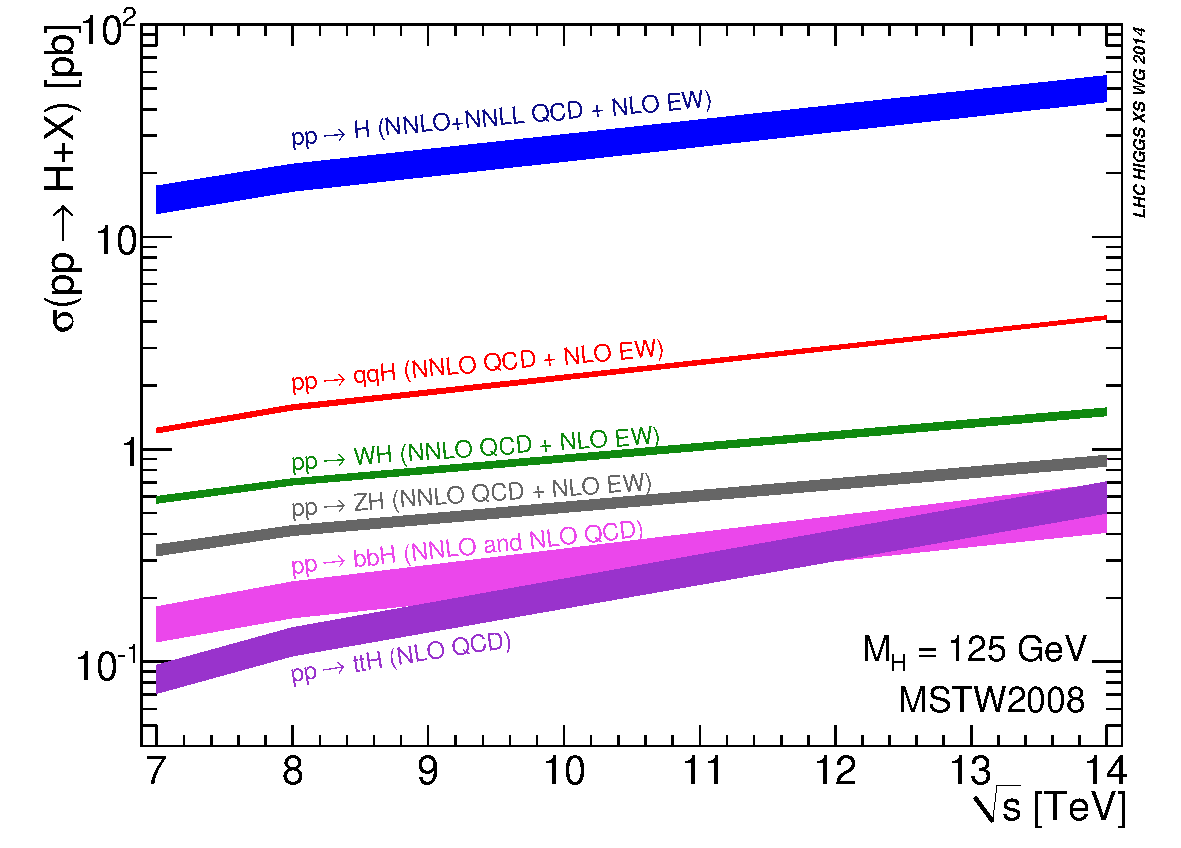
\includegraphics[width=.67\textwidth]{\PhDthesisdir/plots_and_images/from_Higgs_xsec_book_3/Higgs_xsec.pdf}
\caption[Sections efficaces des modes de production du boson de Higgs du modèle standard.]{Sections efficaces des modes de production du boson de Higgs du modèle standard~\cite{Higgs_xsec_book_1,Higgs_xsec_book_2,Higgs_xsec_book_3,Higgs_xsec_book_4}.}
\label{fig-Higgs_xsec}

\vspace{2\baselineskip}

\subcaptionbox{Production par fusion de gluons.\label{subfig-fgraph-gg_loop_h}}[.3\textwidth]
{\begin{fmffile}{gg_loop_h}\fmfstraight
\begin{fmfchar*}(30,20)
  \fmfleft{g1,fi,g2}
  \fmfright{fo1,h,fo2}
  \fmf{gluon}{g1,g1loop}
  \fmf{gluon}{g2,g2loop}
  \fmf{phantom, tension=.6}{g1loop,fo1}
  \fmf{phantom, tension=.6}{g2loop,fo2}
  \fmffreeze
  \fmf{fermion}{g1loop,hloop,g2loop,g1loop}
  \fmf{fermion}{g2loop,g1loop}
  \fmf{dashes, tension=1.75}{hloop,h}
  \fmfdot{g1loop,hloop,g2loop}
  \fmffreeze
  \fmf{phantom}{g1loop,fakev1}
  \fmf{phantom}{g2loop,fakev1}
  \fmffreeze
%  \fmf{phantom,tension=1.5}{hloop,fakev2}
%  \fmf{phantom, label=$t,,\bar{t}$, l.side=left}{fakev1,fakev2}
%  \fmf{phantom, label=$b,,\bar{b}$, l.side=right}{fakev1,fakev2}
  \fmflabel{\gluon}{g1}
  \fmflabel{\gluon}{g2}
  \fmflabel{\higgs}{h}
\end{fmfchar*}
\end{fmffile}
\vspace{\baselineskip}}
\hfill
\subcaptionbox{Production par fusion de bosons vecteurs en voie $t$.\label{subfig-fgraph-Higgs_VBF_t}}[.3\textwidth]
{\begin{fmffile}{Higgs_VBF_t}\fmfstraight
\begin{fmfchar*}(30,20)
  \fmfleft{qa,qb}
  \fmfright{qc,h,qd}
  \fmf{fermion}{qa,v1,qc}
  \fmf{fermion}{qb,v2,qd}
  \fmf{phantom}{qa,v1}
  \fmf{phantom}{qb,v2}
  \fmffreeze
  \fmf{boson, label=$\Wbosonmp,, \Zboson$, l.side=right, tension=3}{v1,v3}
  \fmf{boson, label=$\Wbosonpm,, \Zboson$, l.side=left, tension=3}{v2,v3}
  \fmf{dashes}{v3,h}
  \fmfdot{v1,v2,v3}
  \fmflabel{\quark}{qa}
  \fmflabel{\quark}{qb}
  \fmflabel{\quark}{qc}
  \fmflabel{\quark}{qd}
  \fmflabel{\higgs}{h}
\end{fmfchar*}
\end{fmffile}
\vspace{\baselineskip}}
\hfill
\subcaptionbox{Production par fusion de bosons vecteurs en voie $u$.\label{subfig-fgraph-Higgs_VBF_u}}[.3\textwidth]
{\begin{fmffile}{Higgs_VBF_u}\fmfstraight
\begin{fmfchar*}(42,25)
  \fmfleft{qa,qb}
  \fmfright{qc,h,qd}
  \fmf{fermion}{v1,qc}
  \fmf{fermion}{v2,qd}
  \fmf{phantom,tension=2}{qa,v1}
  \fmf{phantom,tension=2}{qb,v2}
  \fmffreeze
  \fmf{plain}{vv2,v2}
  \fmf{plain}{vv1,v1}
  \fmf{fermion}{qa,vv2}
  \fmf{fermion}{qb,vv1}
  \fmf{boson, label=$\Wbosonpm,, \Zboson$, l.side=right, tension=3}{v1,v3}
  \fmf{boson, label=$\Wbosonpm,, \Zboson$, l.side=left, tension=3}{v2,v3}
  \fmf{dashes}{v3,h}
  \fmfdot{v1,v2,v3}
  \fmflabel{\quark}{qa}
  \fmflabel{\quark}{qb}
  \fmflabel{\quark}{qc}
  \fmflabel{\quark}{qd}
  \fmflabel{\higgs}{h}
\end{fmfchar*}
\end{fmffile}
\vspace{\baselineskip}}
\caption[Production de boson de Higgs par fusion de gluons et de bosons vecteurs.]{Diagrammes de Feynman de production de boson de Higgs dans le cadre du modèle standard par fusion de gluons (\gluon\gluon\higgs) et fusion de bosons vecteurs (VBF).}
\label{fig-fgraph-Higgs_prod_ggh_VBF}

\vspace{2\baselineskip}

\subcaptionbox{Production en association avec un boson \Wboson.\label{subfig-fgraph-Higgs_VH_W}}[.3\textwidth]
{\begin{fmffile}{Higgs_VH_W}\fmfstraight
\begin{fmfchar*}(30,20)
  \fmfleft{i1,i2}
  \fmfright{o1,o2}
  \fmf{fermion}{i1,v1,i2}
  \fmf{boson, label=${\Wbosonpm}^*$, l.side=left}{v1,v2}
  \fmf{boson}{v2,o1}
  \fmf{dashes}{v2,o2}
  \fmfdot{v1,v2}
  \fmflabel{\quark}{i1}
  \fmflabel{\antiquark}{i2}
  \fmflabel{\Wbosonpm}{o1}
  \fmflabel{\higgs}{o2}
\end{fmfchar*}
\end{fmffile}
\vspace{\baselineskip}}
\hfill
\subcaptionbox{Production en association avec un boson \Zboson.\label{subfig-fgraph-Higgs_VH_Z}}[.3\textwidth]
{\begin{fmffile}{Higgs_VH_Z}\fmfstraight
\begin{fmfchar*}(42,25)
  \fmfleft{i1,i2}
  \fmfright{o1,o2}
  \fmf{fermion}{i1,v1,i2}
  \fmf{boson, label=${\Zboson}^*$, l.side=left}{v1,v2}
  \fmf{boson}{v2,o1}
  \fmf{dashes}{v2,o2}
  \fmfdot{v1,v2}
  \fmflabel{\quark}{i1}
  \fmflabel{\antiquark}{i2}
  \fmflabel{\Zboson}{o1}
  \fmflabel{\higgs}{o2}
\end{fmfchar*}
\end{fmffile}
\vspace{\baselineskip}}
\hfill
\subcaptionbox{Production par fusion de gluons associée à un boson \Zboson.\label{subfig-fgraph-Higgs_gg_loop_Zh}}[.3\textwidth]
{\begin{fmffile}{Higgs_gg_loop_Zh}\fmfstraight
\begin{fmfchar*}(42,25)
  \fmfleft{g1,g2}
  \fmfright{Z,h}
  \fmf{gluon}{g1,g1loop}
  \fmf{gluon}{g2,g2loop}
  \fmf{fermion}{g1loop,Zloop,hloop,g2loop,g1loop}
  \fmf{dashes}{hloop,h}
  \fmf{boson}{Zloop,Z}
  \fmfdot{g1loop,Zloop,hloop,g2loop}
  \fmflabel{\gluon}{g1}
  \fmflabel{\gluon}{g2}
  \fmflabel{\higgs}{h}
  \fmflabel{\Zboson}{Z}
\end{fmfchar*}
\end{fmffile}
\vspace{\baselineskip}}
\caption[Production de boson de Higgs en association avec un boson.]{Diagrammes de Feynman de production de boson de Higgs dans le cadre du modèle standard en association avec un boson.}
\label{fig-fgraph-Higgs_prod_VH_ggZh}

\vspace{2\baselineskip}

\subcaptionbox{\label{subfig-fgraph-Higgs_with_t_qq_g_tth}}[.45\textwidth]
{\begin{fmffile}{Higgs_with_t_qq_g_tth}\fmfstraight
\begin{fmfchar*}(30,20)
  \fmfleft{i1,i2}
  \fmfright{o1,o2,o3}
  \fmf{fermion}{i1,v1,i2}
  \fmf{gluon}{v1,v2}
  \fmf{phantom}{o1,v2,o3}
  \fmffreeze
  \fmf{fermion}{o1,v2,v3,o3}
  \fmffreeze
  \fmf{dashes}{v3,o2}
  \fmfdot{v1,v2,v3}
  \fmflabel{\quark}{i1}
  \fmflabel{\antiquark}{i2}
  \fmflabel{\antiquarkt}{o1}
  \fmflabel{\quarkt}{o3}
  \fmflabel{\higgs}{o2}
\end{fmfchar*}
\end{fmffile}
\vspace{\baselineskip}}
\hfill
\subcaptionbox{\label{subfig-fgraph-Higgs_with_t_gg_htt}}[.45\textwidth]
{\begin{fmffile}{gg_htt}\fmfstraight
\begin{fmfchar*}(30,20)
  \fmfleft{g1,g2}
  \fmfright{b1,h,b2}
  \fmf{gluon}{g1,g1b1}
  \fmf{gluon}{g2,g2b2}
  \fmf{fermion}{g1b1,b1}
  \fmf{fermion}{b2,g2b2}
  \fmffreeze
  \fmf{fermion}{g2b2,bh,g1b1}
  \fmffreeze
  \fmf{dashes}{bh,h}
  \fmfdot{g1b1,g2b2,bh}
  \fmflabel{\gluon}{g1}
  \fmflabel{\gluon}{g2}
  \fmflabel{\quarkt}{b1}
  \fmflabel{\antiquarkt}{b2}
  \fmflabel{\higgs}{h}
\end{fmfchar*}
\end{fmffile}
\vspace{\baselineskip}}
\caption[Production de boson de Higgs en association avec un quark~\quarkt.]{Diagrammes de Feynman de production de boson de Higgs dans le cadre du modèle standard en association avec un quark~\quarkt.}
\label{fig-fgraph-Higgs_prod_with_t}
\end{figure}
\subsubsection{Dans le cadre du modèle standard}\label{chapter-MS-MSSM-section-pheno_Higgs_MSSM-subsec-production-SM}
Le mode de production principal du boson de Higgs du modèle standard \higgs\ au LHC est la fusion de gluon, avec près de \SI{85}{\%} des bosons de Higgs produits ainsi.
Ce mode est noté \gluon\gluon\higgs\ et est représenté figure~\ref{subfig-fgraph-gg_loop_h}.
L'interaction entre gluons et Higgs est réalisée par une boucle de quarks.
Le couplage du Higgs aux fermions étant proportionnel à la masse du fermion\footnote{Le lecteur pourra se référer à la section~\ref{chapter-MS-MSSM-section-formalisme-subsec-Higgs_mechanism-subsubsec-fermions}, page~\pageref{chapter-MS-MSSM-section-formalisme-subsec-Higgs_mechanism-subsubsec-fermions}.}, le quark top est dominant dans cette boucle.
\par Le second mode de production de Higgs le plus important au LHC est la fusion de boson vecteur, noté VBF (\emph{Vector Boson Fusion}) et représenté sur les figures~\ref{subfig-fgraph-Higgs_VBF_t} et~\ref{subfig-fgraph-Higgs_VBF_u}.
Deux quarks produisent chacun un boson vecteur (\Wbosonplus\ et \Wbosonminus\ ou deux \Zboson).
Ces deux bosons fusionnent en un boson de Higgs.
Bien que la section efficace du VBF soit dix fois moindre que celle du \gluon\gluon\higgs, les deux quarks de l'état final donnent deux jets\footnote{Le processus de formation de jets à partir de quarks est abordé dans le chapitre\ifref{chapter-JERC}{~\ref{chapter-JERC}}{ \og Calibration en énergie des jets \fg}.} très caractéristiques.
Le calcul de la section efficace de ce processus inclu les corrections QCD\footnote{La chromodynamique quantique (\emph{Quantum ChromoDynamic}) est abordée dans la section~\ref{chapter-MS-MSSM-section-formalisme-subsec-QCD}.} au NNLO\footnote{Les notations NLO, NNLO, N\up{3}LO, etc. signifient \emph{next-to-leading order}, \ie\ jusqu'à l'ordre suivant le premier degré non nul; \emph{next-to-next-to-leading order}, un ordre de plus que NLO; etc.} et les corrections électrofaibles au NLO~\cite{Higgs_xsec_book_4,PhysRevD.85.035002}.
\par La production d'un boson de Higgs peut également se faire en association avec un boson vecteur, c'est le mode VH.
Une paire quark-antiquark produit un boson vecteur de haute énergie (\Wboson\ sur la figure~\ref{subfig-fgraph-Higgs_VH_W} ou \Zboson\ sur la figure~\ref{subfig-fgraph-Higgs_VH_Z}).
Ce boson radie alors un Higgs, d'où la dénomination \og Higgs-strahlung \fg{} parfois utilisée pour le mode VH.
Les sections efficaces de ces processus sont calculées en prenant en compte les corrections QCD NNLO et les corrections électrofaibles au NLO~\cite{Higgs_xsec_book_4}.
Une fusion de gluons peut également amener à une production d'un Higgs en association avec un \Zboson, c'est le cas du processus de la figure~\ref{subfig-fgraph-Higgs_gg_loop_Zh}.
\par Enfin, il est possible de produire un Higgs en association avec des fermions lourds, en particulier des quarks top (\quarkt\antiquarkt\higgs) ou bottom (\quarkb\antiquarkb\higgs) avec lesquels la production de Higgs est accompagnée de jets.
Le mode \quarkt\antiquarkt\higgs\ est illustré sur la figure~\ref{fig-fgraph-Higgs_prod_with_t}.
Ces processus contribuent peu à la production de boson de Higgs au LHC dans le cadre du modèle standard.
Cependant, la phénoménologie du MSSM peut rendre les modes de production en association avec des quarks~\quarkb\ significatifs voire dominants.
\subsubsection{Dans le cadre du MSSM}\label{chapter-MS-MSSM-section-pheno_Higgs_MSSM-subsec-production-MSSM}
Dans la limite découplée du MSSM, compte-tenu des couplages des bosons de Higgs \higgs, \Higgs\ et \HiggsA\ du tableau~\ref{tab-Higgs_couplings_MSSM_decoupling}, les processus présentés dans la section précédente sont modifiés.
Ainsi, la fusion de gluons de la figure~\ref{subfig-fgraph-gg_loop_h} permet, dans le MSSM, de produire \higgs, \Higgs\ et \HiggsA.
Il s'agit toujours du mode dominant tant que $\tan\beta$ ne prend pas de valeur élevée.
Dans le cas de la production de \higgs\ et \Higgs, la boucle peut également contenir des contributions des squarks stop et sbottom s'ils ont des masses suffisamment basses~\cite{Dawson_1996}.
Le mode VBF, dont les processus sont présentés sur les figures~\ref{subfig-fgraph-Higgs_VBF_t} et~\ref{subfig-fgraph-Higgs_VBF_u}, permet de produire \higgs\ et \Higgs, mais pas \HiggsA.
Les corrections aux ordres supérieurs de ces diagrammes dues à la QCD supersymétrique sont faibles et celles dues à la force électrofaible supersymétrique de l'ordre du pourcent~\cite{Higgs_xsec_book_1}.
Ces nouveaux processus sont représentés sur la figure~\ref{fig-fgraph-Higgs_prod_ggh_VBF-MSSM}.
\begin{figure}[h]
\centering
\vspace{\baselineskip}
\subcaptionbox{Production par fusion de gluons.\label{subfig-fgraph-gg_loop_hHA}}[.45\textwidth]
{\begin{fmffile}{gg_loop_hHA}\fmfstraight
\begin{fmfchar*}(42,25)
  \fmfleft{g1,fi,g2}
  \fmfright{fo1,h,fo2}
  \fmf{gluon}{g1,g1loop}
  \fmf{gluon}{g2,g2loop}
  \fmf{phantom, tension=.6}{g1loop,fo1}
  \fmf{phantom, tension=.6}{g2loop,fo2}
  \fmffreeze
  \fmf{fermion}{g1loop,hloop,g2loop,g1loop}
  \fmf{fermion}{g2loop,g1loop}
  \fmf{dashes, label=$\Hs,, \Hn,, \Ha$, l.side=left, tension=1.75}{hloop,h}
  \fmfdot{g1loop,hloop,g2loop}
  \fmffreeze
  \fmf{phantom}{g1loop,fakev1}
  \fmf{phantom}{g2loop,fakev1}
  \fmffreeze
%  \fmf{phantom,tension=1.5}{hloop,fakev2}
%  \fmf{phantom, label=$t,,\bar{t}$, l.side=left}{fakev1,fakev2}
%  \fmf{phantom, label=$b,,\bar{b}$, l.side=right}{fakev1,fakev2}
  \fmflabel{\gluon}{g1}
  \fmflabel{\gluon}{g2}
\end{fmfchar*}
\end{fmffile}
\vspace{\baselineskip}}
\hfill
\subcaptionbox{Production par fusion de bosons vecteurs en voie $t$.\label{subfig-fgraph-Higgs_VBF_t-MSSM}}[.45\textwidth]
{\begin{fmffile}{Higgs_VBF_t-MSSM}\fmfstraight
\begin{fmfchar*}(30,20)
  \fmfleft{qa,qb}
  \fmfright{qc,h,qd}
  \fmf{fermion}{qa,v1,qc}
  \fmf{fermion}{qb,v2,qd}
  \fmf{phantom}{qa,v1}
  \fmf{phantom}{qb,v2}
  \fmffreeze
  \fmf{boson, label=$\Wbosonmp,, \Zboson$, l.side=right, tension=3}{v1,v3}
  \fmf{boson, label=$\Wbosonpm,, \Zboson$, l.side=left, tension=3}{v2,v3}
  \fmf{dashes}{v3,h}
  \fmfdot{v1,v2,v3}
  \fmflabel{\quark}{qa}
  \fmflabel{\quark}{qb}
  \fmflabel{\quark}{qc}
  \fmflabel{\quark}{qd}
  \fmflabel{\higgs, \Higgs}{h}
\end{fmfchar*}
\end{fmffile}
\vspace{\baselineskip}}
\caption[Production de boson de Higgs du MSSM par fusion de gluons et de bosons vecteurs.]{Diagrammes de Feynman de production de boson de Higgs dans le cadre du MSSM par fusion de gluons (\gluon\gluon\Higgs) et fusion de bosons vecteurs (VBF).}
\label{fig-fgraph-Higgs_prod_ggh_VBF-MSSM}
\end{figure}
\par Dans le mode VH, le Higgs radié peut également être un \Higgs.
Les processus de la figure~\ref{fig-fgraph-Higgs_prod_VH_ggZh} sont ainsi modifiés en ceux de la figure~\ref{fig-fgraph-Higgs_prod_VH_ggZh-MSSM}.
Les corrections aux ordres supérieurs de ces diagrammes dues à la QCD supersymétrique sont faibles et celles dues à la force électrofaible supersymétrique ne sont pas connues~\cite{Higgs_xsec_book_1}.
\begin{figure}[h]
\centering
\vspace{\baselineskip}
\subcaptionbox{Production en association avec un boson \Wboson.\label{subfig-fgraph-Higgs_VH_W-MSSM}}[.45\textwidth]
{\begin{fmffile}{Higgs_VH_W-MSSM}\fmfstraight
\begin{fmfchar*}(30,20)
  \fmfleft{i1,i2}
  \fmfright{o1,o2}
  \fmf{fermion}{i1,v1,i2}
  \fmf{boson, label=${\Wbosonpm}^*$, l.side=left}{v1,v2}
  \fmf{boson}{v2,o1}
  \fmf{dashes}{v2,o2}
  \fmfdot{v1,v2}
  \fmflabel{\quark}{i1}
  \fmflabel{\antiquark}{i2}
  \fmflabel{\Wbosonpm}{o1}
  \fmflabel{\higgs, \Higgs}{o2}
\end{fmfchar*}
\end{fmffile}
\vspace{\baselineskip}}
\hfill
\subcaptionbox{Production en association avec un boson \Zboson.\label{subfig-fgraph-Higgs_VH_Z-MSSM}}[.45\textwidth]
{\begin{fmffile}{Higgs_VH_Z-MSSM}\fmfstraight
\begin{fmfchar*}(30,20)
  \fmfleft{i1,i2}
  \fmfright{o1,o2}
  \fmf{fermion}{i1,v1,i2}
  \fmf{boson, label=${\Zboson}^*$, l.side=left}{v1,v2}
  \fmf{boson}{v2,o1}
  \fmf{dashes}{v2,o2}
  \fmfdot{v1,v2}
  \fmflabel{\quark}{i1}
  \fmflabel{\antiquark}{i2}
  \fmflabel{\Zboson}{o1}
  \fmflabel{\higgs, \Higgs}{o2}
\end{fmfchar*}
\end{fmffile}
\vspace{\baselineskip}}
\caption[Production de boson de Higgs du MSSM en association avec un boson.]{Diagrammes de Feynman de production de boson de Higgs dans le cadre du MSSM en association avec un boson.}
\label{fig-fgraph-Higgs_prod_VH_ggZh-MSSM}
\end{figure}
\par Pour de grandes valeurs de $\tan\beta$, la production de Higgs lourds en association avec des quarks~\quarkb\ est un mode dominant.
Plusieurs processus participent à ce mode.
Sur les figures~\ref{subfig-fgraph-Higgs_with_b_qq_g_bbh-MSSM} et~\ref{subfig-fgraph-gg_hHAbb} se trouvent les processus analogues à ceux du mode \quarkt\antiquarkt\higgs\ du modèle standard présentés figures~\ref{subfig-fgraph-Higgs_with_t_qq_g_tth} et~\ref{subfig-fgraph-Higgs_with_t_gg_htt}.
Des processus comme ceux des figures~\ref{subfig-fgraph-bb_hHA} et~\ref{subfig-fgraph-bg_b_bhHA} sont également envisageables si le quark~\quarkb\ est considéré comme présent au sein du proton, c'est le \og schéma à cinq saveurs \fg{} ou 5fs (\emph{5-flavor scheme}).
Les sections efficaces des processus du mode \quarkb\antiquarkb\higgs\ sont calculées au NLO dans le 4fs et au NNLO pour le 5fs.
\par Les processus des figures~\ref{subfig-fgraph-Higgs_with_b_qq_g_bbh-MSSM} et~\ref{subfig-fgraph-gg_hHAbb} présentent deux jets de quarks~\quarkb\ associés à la production d'un boson de Higgs, celui de la figure~\ref{subfig-fgraph-bg_b_bhHA} un jet de quark~\quarkb.
L'identification de ces jets est donc un enjeu dans les analyses testant les cas de hautes valeurs de $\tan\beta$.
\begin{figure}[h]
\centering
\vspace{\baselineskip}
\subcaptionbox{\label{subfig-fgraph-Higgs_with_b_qq_g_bbh-MSSM}}[.45\textwidth]
{\begin{fmffile}{qq_g_bbhHA}\fmfstraight
\begin{fmfchar*}(30,20)
  \fmfleft{i1,i2}
  \fmfright{o1,o2,o3}
  \fmf{fermion}{i1,v1,i2}
  \fmf{gluon}{v1,v2}
  \fmf{phantom}{o1,v2,o3}
  \fmffreeze
  \fmf{fermion}{o1,v2,v3,o3}
  \fmffreeze
  \fmf{dashes}{v3,o2}
  \fmfdot{v1,v2,v3}
  \fmflabel{\quark}{i1}
  \fmflabel{\antiquark}{i2}
  \fmflabel{\antiquarkb}{o1}
  \fmflabel{\quarkb}{o3}
  \fmflabel{\higgs, \Higgs, \HiggsA}{o2}
\end{fmfchar*}
\end{fmffile}
\vspace{\baselineskip}}
\hfill
\subcaptionbox{\label{subfig-fgraph-gg_hHAbb}}[.45\textwidth]
{\begin{fmffile}{gg_hHAbb}\fmfstraight
\begin{fmfchar*}(30,20)
  \fmfleft{g1,g2}
  \fmfright{b1,h,b2}
  \fmf{gluon}{g1,g1b1}
  \fmf{gluon}{g2,g2b2}
  \fmf{fermion}{g1b1,b1}
  \fmf{fermion}{b2,g2b2}
  \fmffreeze
  \fmf{fermion}{g2b2,bh,g1b1}
  \fmffreeze
  \fmf{dashes, label=$\Hs,, \Hn,, \Ha$, l.side=left}{bh,h}
  \fmfdot{g1b1,g2b2,bh}
  \fmflabel{\gluon}{g1}
  \fmflabel{\gluon}{g2}
  \fmflabel{\quarkb}{b1}
  \fmflabel{\antiquarkb}{b2}
\end{fmfchar*}
\end{fmffile}
\vspace{\baselineskip}}

\vspace{2\baselineskip}
\subcaptionbox{\label{subfig-fgraph-bb_hHA}}[.45\textwidth]
{\begin{fmffile}{bb_hHA}\fmfstraight
\begin{fmfchar*}(30,20)
  \fmfleft{b1,b2}
  \fmfright{h}
  \fmf{fermion}{b1,bh}
  \fmf{fermion}{bh,b2}
  \fmf{dashes, label=$\Hs,, \Hn,, \Ha$, l.side=left}{bh,h}
  \fmfdot{bh}
  \fmflabel{\quarkb}{b1}
  \fmflabel{\antiquarkb}{b2}
\end{fmfchar*}
\end{fmffile}
\vspace{\baselineskip}}
\hfill
\subcaptionbox{\label{subfig-fgraph-bg_b_bhHA}}[.45\textwidth]
{\begin{fmffile}{bg_b_bhHA}\fmfstraight
\begin{fmfchar*}(42,25)
  \fmfleft{i1,i2}
  \fmfright{o1,o2}
  \fmf{fermion}{i2,v1,v2,o1}
  \fmf{gluon}{i1,v1}
  \fmf{dashes, label=$\Hs,, \Hn,, \Ha$, l.side=left}{v2,o2}
  \fmfdot{v1,v2}
  \fmflabel{\gluon}{i1}
  \fmflabel{\quarkb}{i2}
  \fmflabel{\quarkb}{o1}
\end{fmfchar*}
\end{fmffile}\vspace{\baselineskip}}

\caption[Production de boson de Higgs du MSSM en association avec un quark~\quarkb.]{Diagrammes de Feynman de production de boson de Higgs dans le cadre du MSSM en association avec un quark~\quarkb.}
\label{fig-fgraph-Higgs_prod_with_b-MSSM}
\end{figure}
\subsection{Désintégration de bosons de Higgs}\label{chapter-MS-MSSM-section-pheno_Higgs_MSSM-subsec-desintegration_Higgs}
\begin{figure}[p]
\centering
\subcaptionbox{Rapports de branchement à $\tan\beta=5$ pour \higgs.\label{subfig-BR_h_tanbeta_5}}[.45\textwidth]
{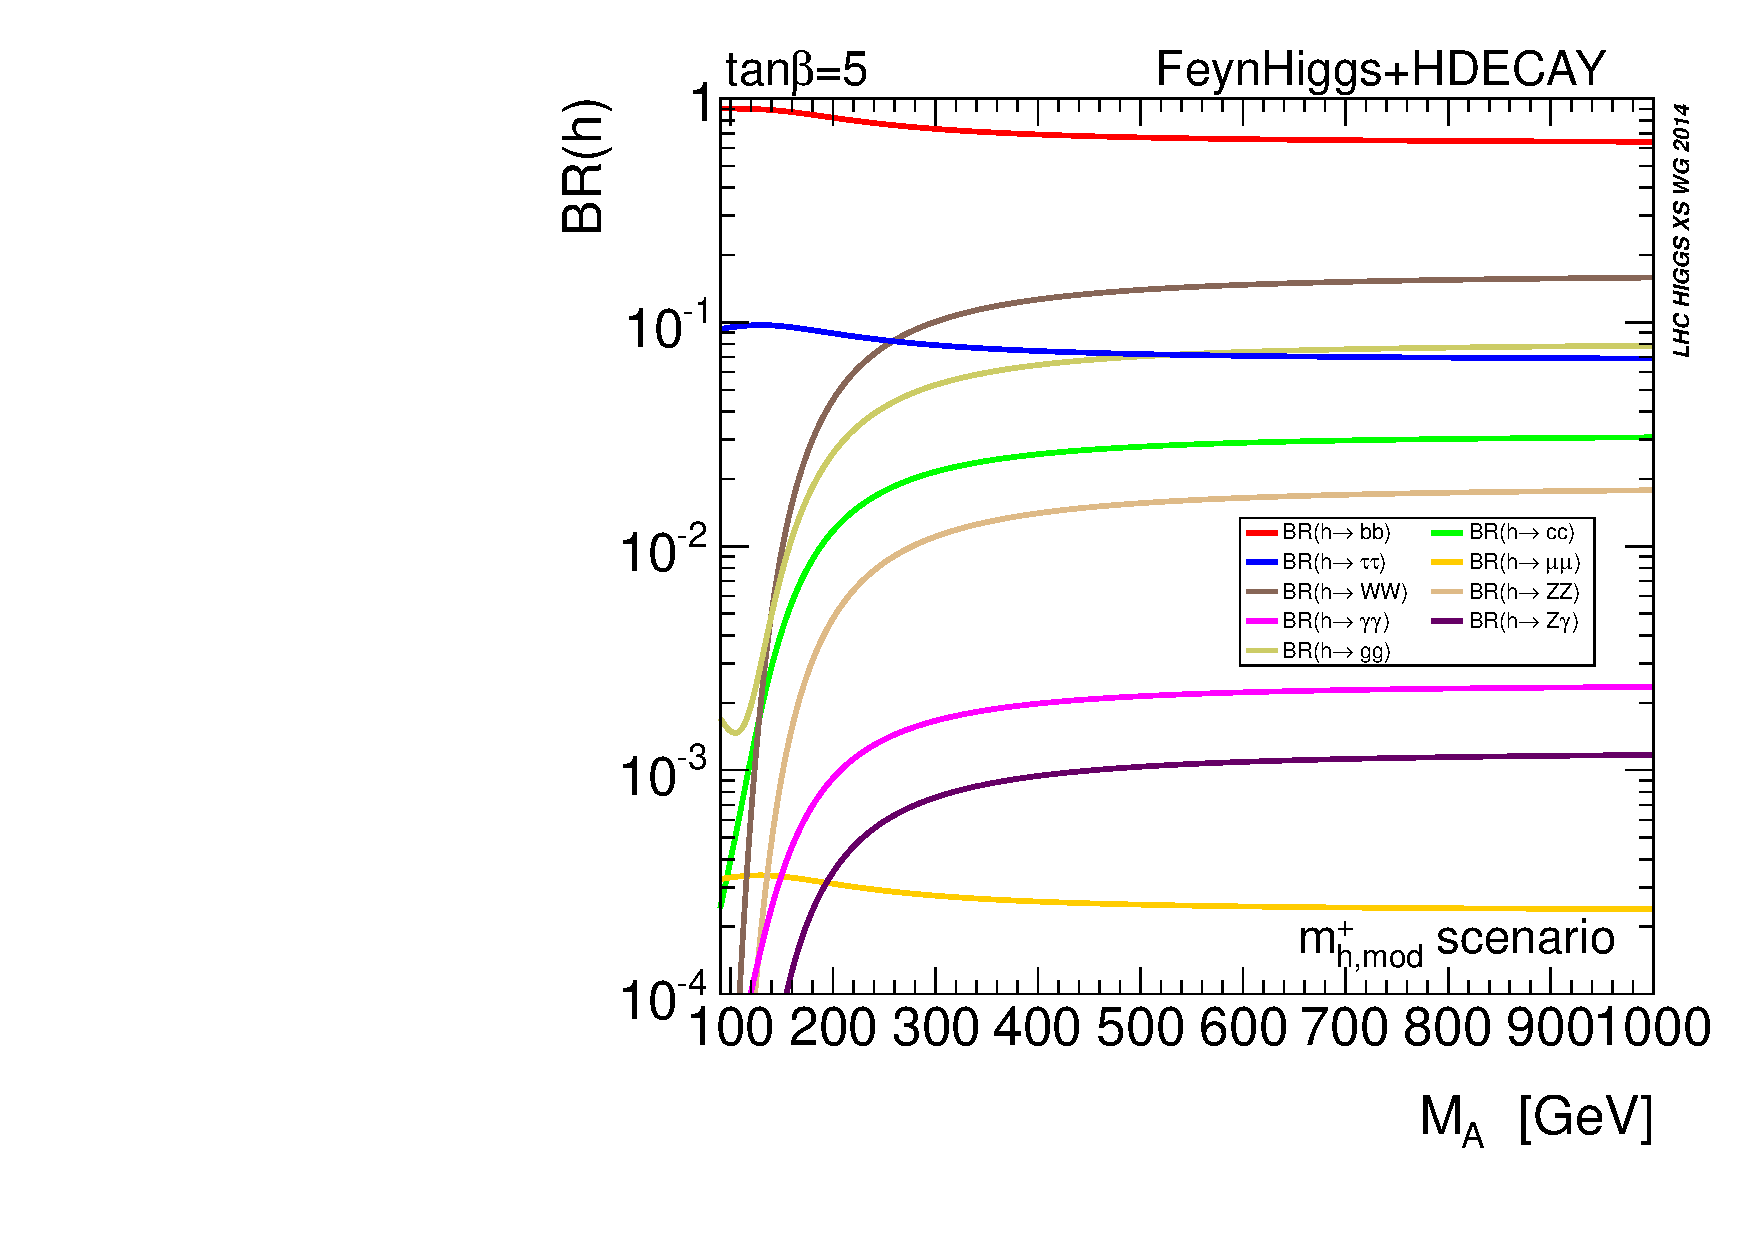
\includegraphics[width=.45\textwidth]{\PhDthesisdir/plots_and_images/from_Higgs_xsec_book_3/YR4HXS_BRSummary_h_mhmodp_tanbeta5_FeynHiggs_HDecay}\vspace{-.5\baselineskip}}
\hfill
\subcaptionbox{Rapports de branchement à $\tan\beta=30$ pour \higgs.\label{subfig-BR_h_tanbeta_30}}[.45\textwidth]
{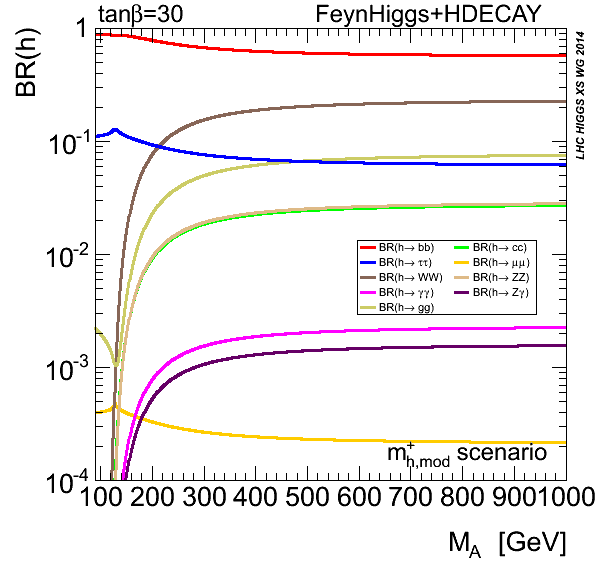
\includegraphics[width=.45\textwidth]{\PhDthesisdir/plots_and_images/from_Higgs_xsec_book_3/YR4HXS_BRSummary_h_mhmodp_tanbeta30_FeynHiggs_HDecay}\vspace{-.5\baselineskip}}

\vspace{.75\baselineskip}
\subcaptionbox{Rapports de branchement à $\tan\beta=5$ pour \Higgs.\label{subfig-BR_H_tanbeta_5}}[.45\textwidth]
{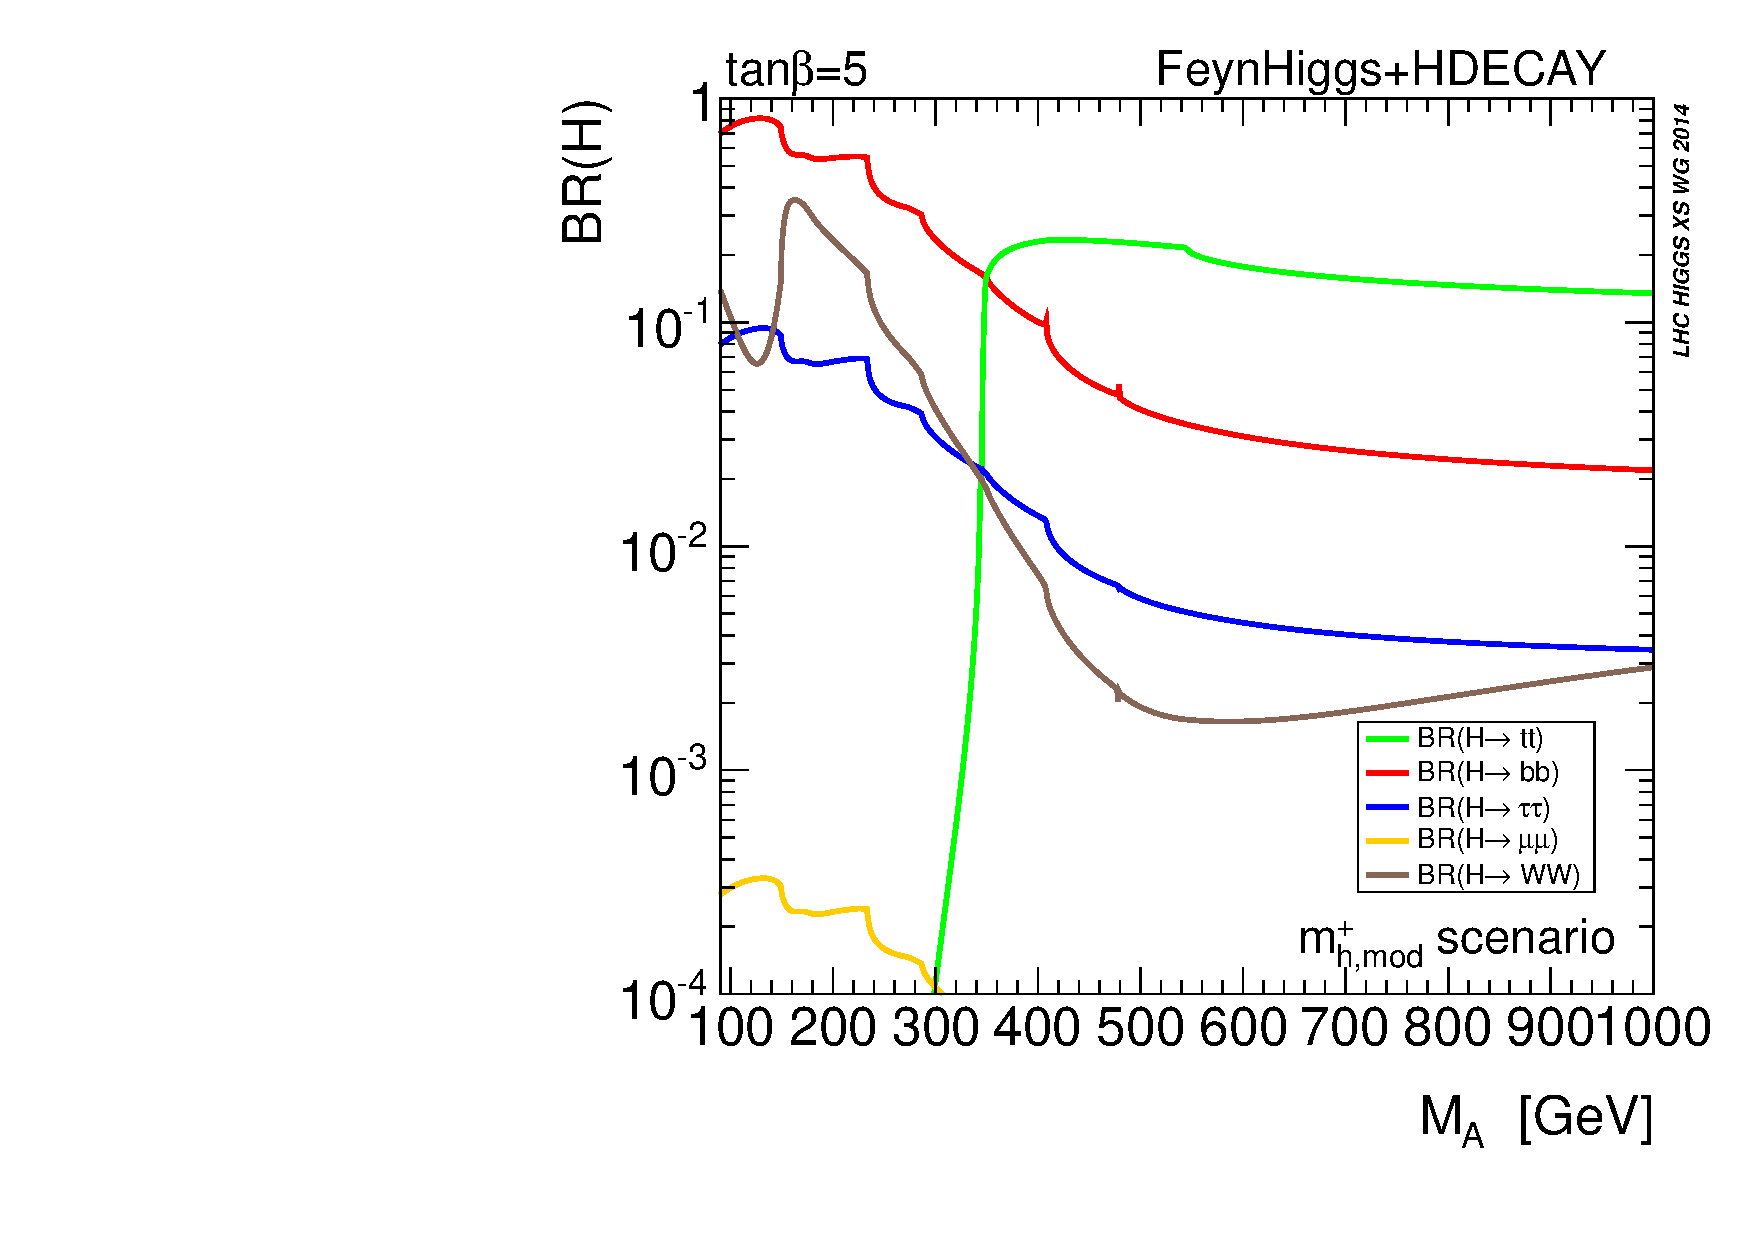
\includegraphics[width=.45\textwidth]{\PhDthesisdir/plots_and_images/from_Higgs_xsec_book_3/YR4HXS_BRSummary_H_mhmodp_tanbeta5_FeynHiggs_HDecay}\vspace{-.5\baselineskip}}
\hfill
\subcaptionbox{Rapports de branchement à $\tan\beta=30$ pour \Higgs.\label{subfig-BR_H_tanbeta_30}}[.45\textwidth]
{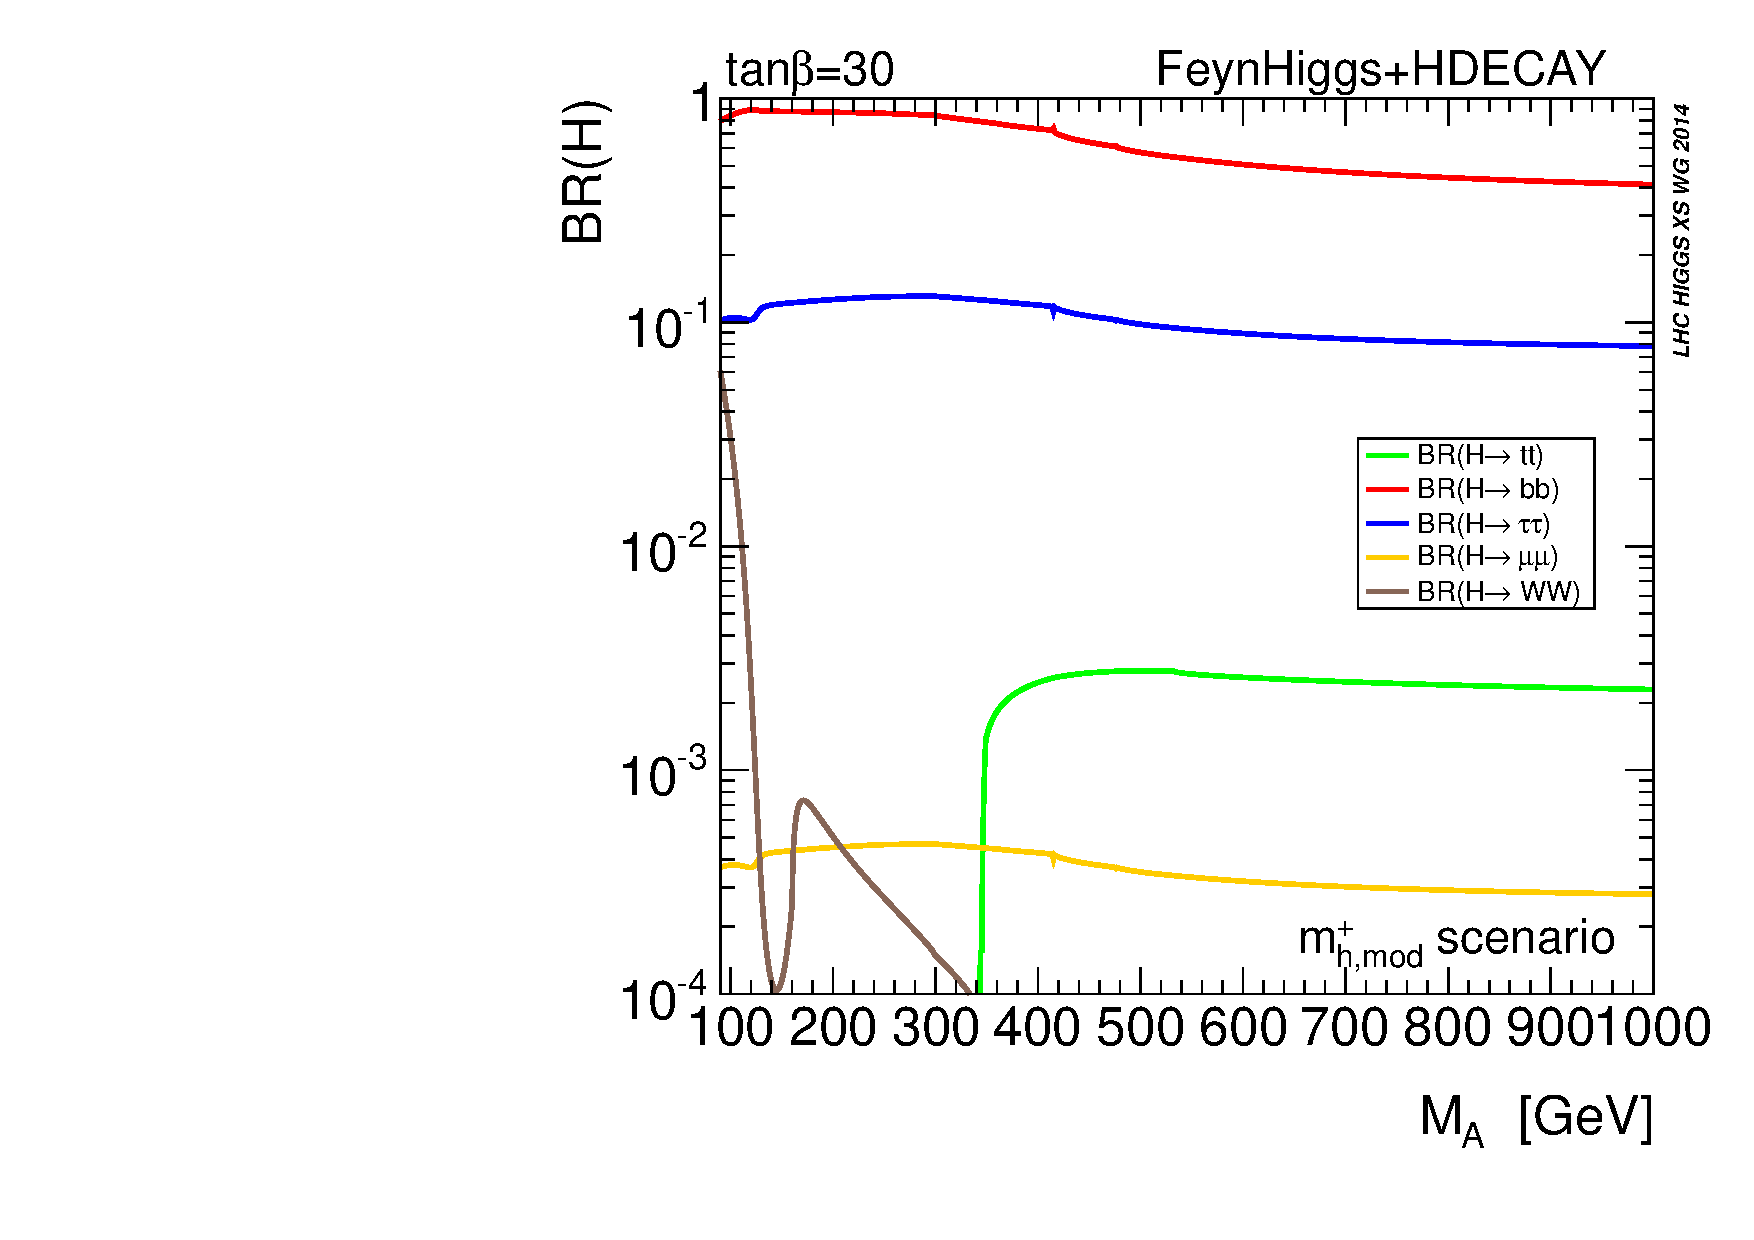
\includegraphics[width=.45\textwidth]{\PhDthesisdir/plots_and_images/from_Higgs_xsec_book_3/YR4HXS_BRSummary_H_mhmodp_tanbeta30_FeynHiggs_HDecay}\vspace{-.5\baselineskip}}

\vspace{.75\baselineskip}
\subcaptionbox{Rapports de branchement à $\tan\beta=5$ pour \HiggsA.\label{subfig-BR_A_tanbeta_5}}[.45\textwidth]
{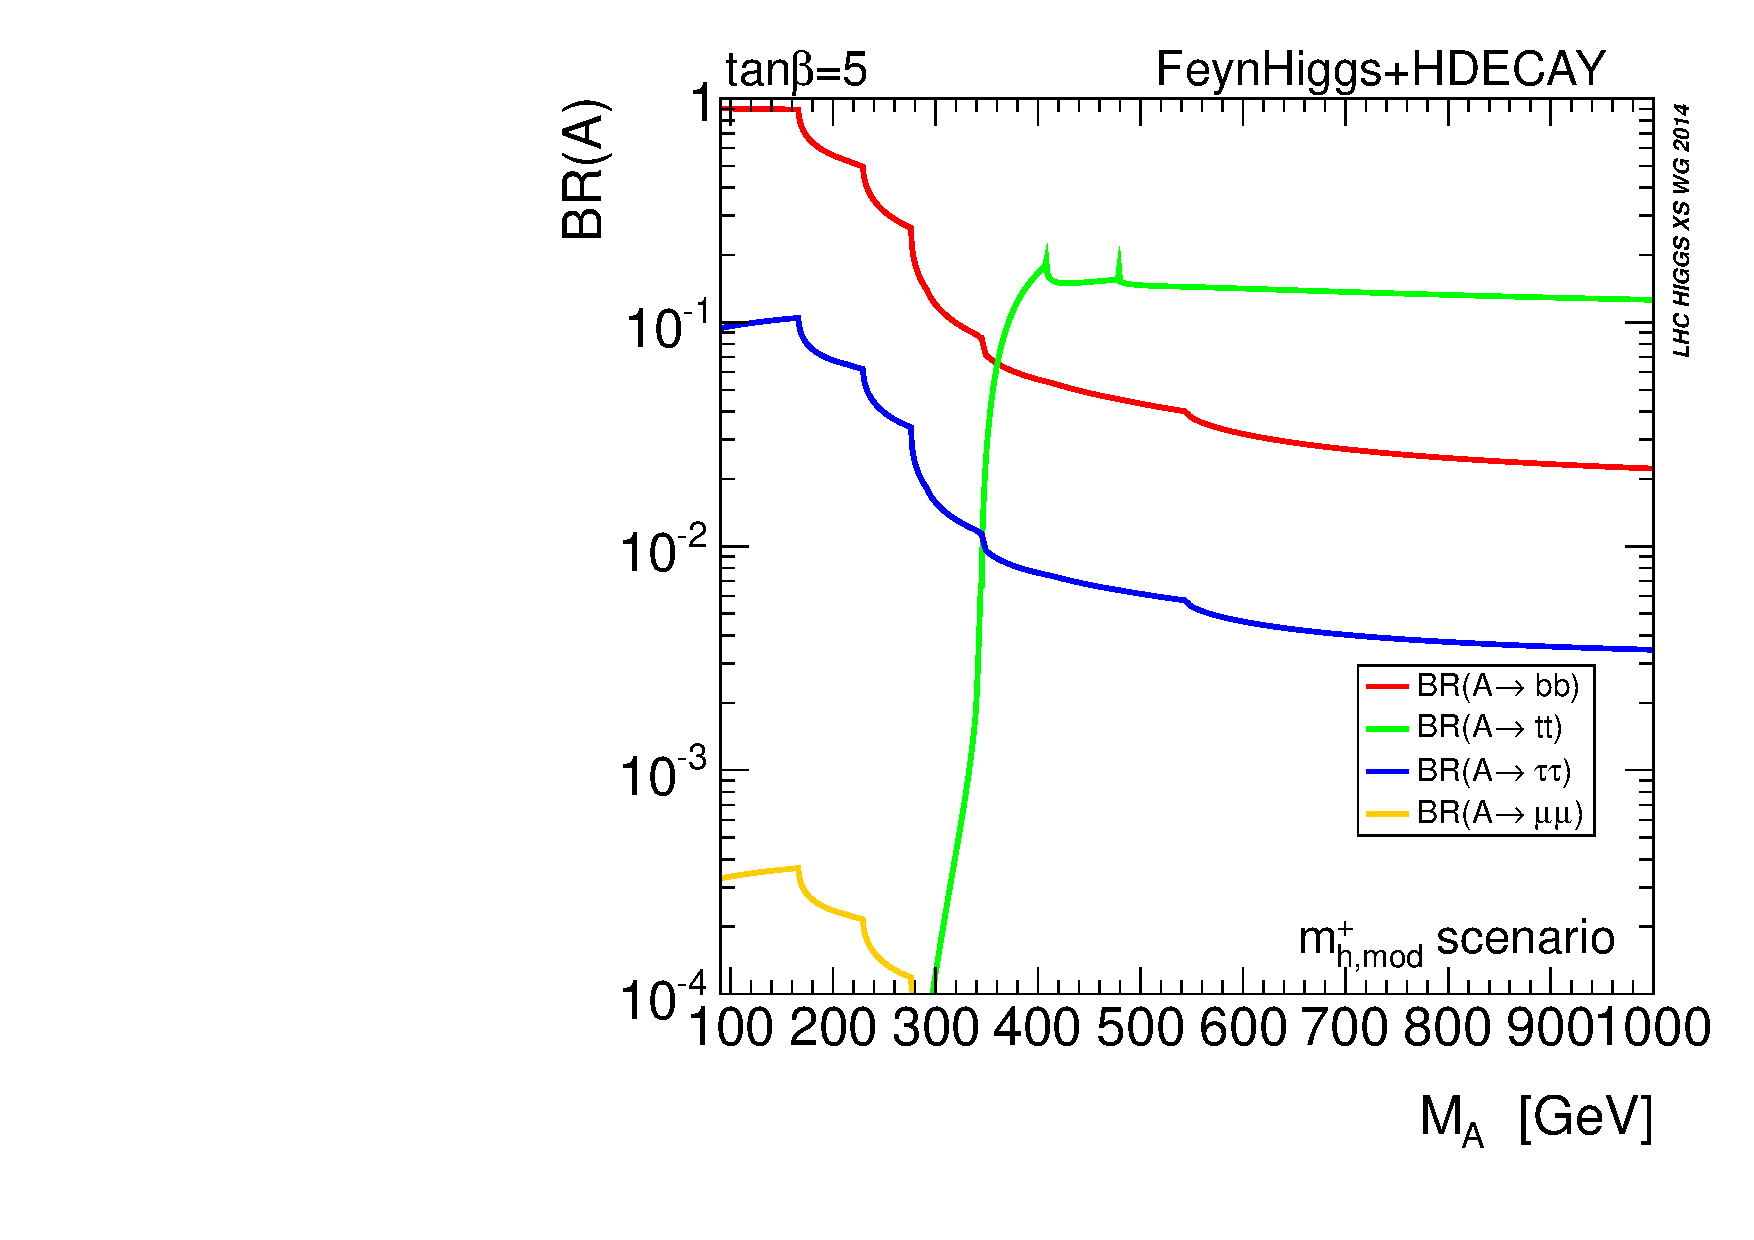
\includegraphics[width=.45\textwidth]{\PhDthesisdir/plots_and_images/from_Higgs_xsec_book_3/YR4HXS_BRSummary_A_mhmodp_tanbeta5_FeynHiggs_HDecay}\vspace{-.5\baselineskip}}
\hfill
\subcaptionbox{Rapports de branchement à $\tan\beta=30$ pour \HiggsA.\label{subfig-BR_A_tanbeta_30}}[.45\textwidth]
{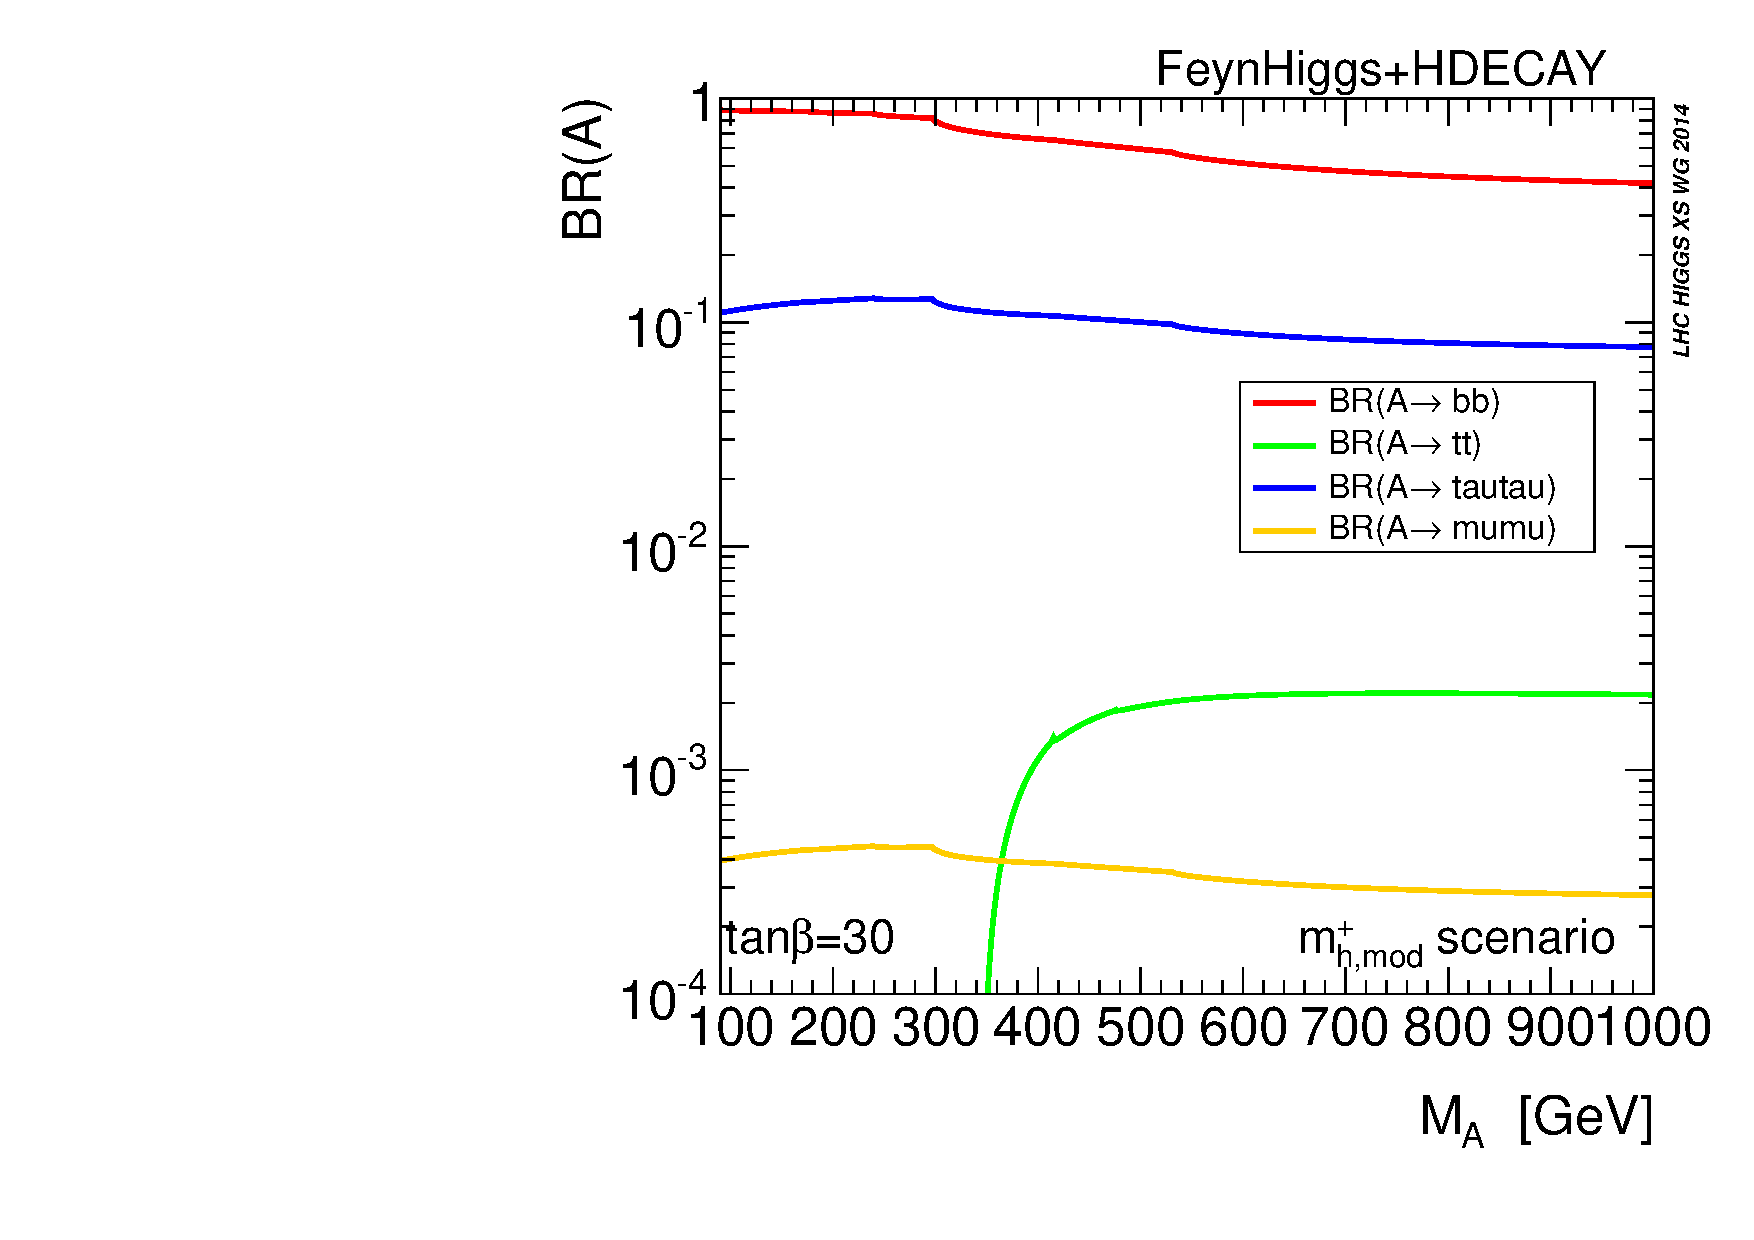
\includegraphics[width=.45\textwidth]{\PhDthesisdir/plots_and_images/from_Higgs_xsec_book_3/YR4HXS_BRSummary_A_mhmodp_tanbeta30_FeynHiggs_HDecay}\vspace{-.5\baselineskip}}

\caption[Rapports de branchement des bosons de Higgs du MSSM.]{Rapports de branchement des bosons de Higgs du MSSM en fonction de $m_{\HiggsA}$ pour $\tan\beta=5$ et $30$~\cite{Higgs_xsec_book_2,Higgs_xsec_book_3}. L'effet de $\tan\beta$ sur les couplages de \Higgs\ et \HiggsA\ aux fermions est bien visible avec l'augmentation des rapports de branchement au bottom (en rouge) et au tau (en bleu) et la diminution du rapport de branchement au top (en vert).}
\label{fig-BR_hHA_tanbeta_5_30}
\end{figure}
Les bosons de Higgs ont une durée de vie très courte, de l'ordre de \SI{e-22}{\second} pour le boson de Higgs du modèle standard par exemple~\cite{PDG_booklet_2020}.
Leur propagation se fait ainsi sur des distances ne pouvant excéder quelques dizaines de femtomètres, \ie\ \SI{e-14}{\meter}, soit moins que le diamètre du noyau d'un atome d'or.
Il est donc impossible d'observer directement la présence d'un boson de Higgs, comme cela peut se faire avec d'autres particules plus stables comme les kaons, les muons, les électrons ou les protons pour ne citer qu'eux.
Pour détecter ces bosons, il faut donc détecter leurs produits de désintégration.
\par La désintégration des bosons de Higgs peut se faire sous différentes formes ayant différents rapports de branchement ou \BR{} (\emph{Branching Ratio}), \ie\ différentes probabilités de survenir vis-à-vis des autres formes.
La topologie des événements correspondants est également fortement affectée par les produits de désintégration des bosons de Higgs.
\par Les bosons de Higgs supplémentaires \Higgs\ et \HiggsA\ voient leurs couplages aux bosons vecteurs supprimés dans la limite découplée du MSSM.
Leurs couplages sont proportionnels à $\tan\beta$ avec les fermions d'isospin faible bas et inversement proportionnels à $\tan\beta$ avec les fermions d'isospin faible haut par rapport au couplage de \higgs\ avec ces mêmes fermions.
Les couplages des bosons de Higgs aux fermions sont de plus proportionnels aux masses de ces fermions.
Ces rapports de branchement sont représentés sur la figure~\ref{fig-BR_hHA_tanbeta_5_30}, page~\pageref{fig-BR_hHA_tanbeta_5_30}, pour les trois bosons de Higgs neutres du MSSM et pour $\tan\beta=5$ et $30$.
Pour des masses de \Higgs\ et \HiggsA\ suffisamment grandes pour leur permettre de se désintégrer en paire de quarks~\quarkt, malgré la masse élevée de ce dernier, la suppression des couplages aux fermions d'isospin faible haut par $\tan\beta$ laisse le quark~\quarkb\ et le lepton~\tau\ avec les rapports de branchement les plus élevés à haut $\tan\beta$.
Les rapports de branchement du boson de Higgs \higgs\ correspondant au boson de Higgs du modèle standard sont peu affectés par $\tan\beta$.
\par La valeur de $\tan\beta$ est un paramètre libre du MSSM pouvant être grand.
À haut $\tan\beta$ le quark~\quarkb\ et le lepton~\tau\ proposent les rapports de branchement les plus grands à \Higgs\ et \HiggsA.
Pour des valeurs modérées voire basses de $\tan\beta$, le quark top peut éventuellement proposer un rapport de branchement plus grand, mais seulement pour $m_{\HiggsA}\gtrsim\SI{350}{\GeV}$.
Les désintégrations en \quarkb\antiquarkb\ et en \antitau\leptau\ sont donc les plus prometteuses pour la recherche de bosons de Higgs supplémentaires de haute masse.
\par Bien que le canal de désintégration $\higgs,\Higgs,\HiggsA \to \quarkb\antiquarkb$ possède un rapport de branchement 5 à 10 fois supérieur à celui du canal $\higgs,\Higgs,\HiggsA \to \antitau\leptau$, il est sujet à de nombreuses sources de bruit de fond au LHC où les collisions ont lieu entre protons.
C'est pourquoi le sujet de cette thèse est la recherche d'un boson de Higgs de haute masse se désintégrant en paire de taus, dont l'accessibilité expérimentale est meilleure.
La présence de deux leptons tau de haute énergie dans l'état final est en effet une signature bien plus claire que la présence de quarks~\quarkb.
Le diagramme de Feynman correspondant à cette désintégration est présenté sur la figure~\ref{fig-H_to_tau_tau_fmf_graph_1}.
Toutefois, les taus ne sont pas des particules stables et ils se désintègrent avant d'entrer dans les parties sensibles du détecteur.
Seuls leurs produits de désintégration sont observés.
\begin{figure}[h]
\centering
\begin{fmffile}{H-tautau_small}\fmfstraight
\begin{fmfchar*}(40,30)
  \fmfleft{h}
  \fmfright{tau1,tau2}
  \fmf{dashes, label=$\Hs,, \Hn,, \Ha$, l.side=left}{h,v}
  \fmf{fermion, label=$\tau^+$, l.side=left}{tau1,v}
  \fmf{fermion, label=$\tau^-$, l.side=left}{v,tau2}
  \fmfdot{v}
\end{fmfchar*}
\end{fmffile}
\vspace{\baselineskip}
\caption[Désintégration $\higgs, \Higgs, \HiggsA \to \antitau\leptau$.]{Diagramme de Feynman d'une désintégration $\higgs, \Higgs, \HiggsA \to \antitau\leptau$.}
\label{fig-H_to_tau_tau_fmf_graph_1}
\end{figure}
\subsection{Désintégration des leptons tau}\label{chapter-MS-MSSM-section-pheno_Higgs_MSSM-subsec-desintegration_lepton_tau}
La durée de vie du lepton \tau\ est de \SI{290}{\femto\second}. Ils se propage ainsi sur des distances inférieures à \SI{87}{\micro\meter}.
Le \tau\ n'est donc pas directement observé dans le détecteur, ses produits de désintégration le sont.
\par Les leptons \tau\ se désintègrent par interaction faible selon $\leptau\to\Wbosonminus\nutau$.
Le boson \Wboson, virtuel, se désintègre ensuite:
\begin{itemize}
\item leptoniquement selon $\Wbosonminus\to\electron\antinuele$ dans \SI{17.82}{\%} des cas;
\item leptoniquement selon $\Wbosonminus\to\muon\antinumu$ dans \SI{17.39}{\%} des cas;
\item hadroniquement selon $\Wbosonminus\to\quark\antiquark'$ dans \SI{64.79}{\%} des cas.
\end{itemize}
\par Dans le cas de la désintégration hadronique, le phénomène de hadronisation\footnote{L'hadronisation est présentée dans la section~\ifref{chapter-JERC-section-jets-subsec-hadronisation}{\ref{chapter-JERC-section-jets-subsec-hadronisation}}{2.2} du chapitre\ifref{chapter-JERC}{~\ref{chapter-JERC}}{ \og Calibration en énergie des jets \fg{}}.} a lieu et les deux quarks donnent un ensemble constitué de quelques hadrons, en général trois ou moins, et éventuellement des particules neutres comme des \pionnull, ces derniers se désintégrant majoritairement en deux photons.
L'ensemble des particules issues de la désintégration du \Wboson\ forme ainsi un petit jet.
Il s'agit d'un \og tau hadronique \fg, noté \tauh\ dans la suite.
\par Les diagrammes de Feynman correspondant aux désintégrations leptonique et hadronique du \tau\ sont représentés figures~\ref{subfig-fgraph-tau_to_ell} et~\ref{subfig-fgraph-tau_to_tauh}.
Le tableau~\ref{subtab-tau_decay_modes_BRs} résume plus en détails les rapports de branchement des différents modes de désintégration du \tau.
\begin{figure}[h]
\centering
\vspace{\baselineskip}
\subcaptionbox{Désintégration leptonique d'un \leptau. Le lepton $\ell$ peut être un électron ou un muon.\label{subfig-fgraph-tau_to_ell}}[.45\textwidth]
{\begin{fmffile}{tau_to_ell}%\fmfstraight
\begin{fmfchar*}(30,20)
  \fmfleft{taui}
  \fmfright{l1,l2,l3,f1,f2,f3,nuout}
  \fmf{fermion, tension=2}{taui,v1}
  \fmf{fermion}{v1,nuout}
  \fmf{phantom}{v1,l1}
  \fmffreeze
  \fmflabel{$\nutau$}{nuout}
  \fmf{boson, label=$\Wbosonminus$, l.side=right, tension=2}{v1,v2}
  \fmf{phantom}{v2,td1,l1}
  \fmf{phantom}{v2,td2,l2}
  \fmf{phantom}{v2,td3,l3}
  \fmffreeze
  \fmf{fermion}{l1,v2,l3}
  \fmflabel{$\antineutrino_\ell$}{l1}
  \fmflabel{$\ell$}{l3}
  \fmflabel{\leptau}{taui}
  \fmfdot{v1,v2}
\end{fmfchar*}
\end{fmffile}
\vspace{\baselineskip}}
\hfill
\subcaptionbox{Désintégration hadronique d'un \leptau.\label{subfig-fgraph-tau_to_tauh}}[.45\textwidth]
{\begin{fmffile}{tau_to_tauh_small_beamer}%\fmfstraight
\begin{fmfchar*}(20,10)
  \fmfleft{taui}
  \fmfright{l1,l2,l3,f1,f2,f3,nuout}
  \fmf{fermion, tension=2}{taui,v1}
  \fmf{fermion}{v1,nuout}
  \fmf{phantom}{v1,l1}
  \fmffreeze
  \fmflabel{$\nutau$}{nuout}
  \fmf{boson, label=$\Wbosonminus$, l.side=right, tension=2}{v1,v2}
  \fmf{phantom}{v2,td1,l1}
  \fmf{phantom}{v2,td2,l2}
  \fmf{phantom}{v2,td3,l3}
  \fmffreeze
  \fmf{plain}{td3,v2,td1}
  \fmfblob{.15w}{td2}
  \fmf{plain}{td2,l2}
  \fmflabel{\tauhm}{l2}
  \fmflabel{\leptau}{taui}
  \fmfdot{v1,v2}
\end{fmfchar*}
\end{fmffile}
\vspace{\baselineskip}}
\caption{Diagrammes de Feynman de désintégration d'un \leptau.}
\label{fig-fgraph-tau_to_ell_and_tauh}
\end{figure}
\begin{table}[h]
\centering
\subcaptionbox{Rapports de branchement des différents modes de désintégration du \tau~\cite{PDG_booklet_2020}.\label{subtab-tau_decay_modes_BRs}}[.45\textwidth]
{\begin{tabular}{lc}
\toprule
Mode de désintégration & \BR{} (\SI{}{\%})\\
\midrule
$\leptau\to \electron\antinuele\antinutau$ & \num{17.82} \\
$\leptau\to \muon\antinumu\antinutau$ & \num{17.39} \\
\midrule
$\leptau\to \hadronminus \antinutau$ & \num{11.51} \\
$\leptau\to \hadronminus \pionnull \antinutau$ & \num{25.93} \\
$\leptau\to \hadronminus \pionnull\pionnull \antinutau$ & \num{9.48} \\
$\leptau\to \hadronminus \hadronminus\hadronplus \antinutau$ & \num{9.80} \\
$\leptau\to \hadronminus \hadronminus\hadronplus\pionnull\antinutau$ & \num{4.76} \\
Autres modes hadroniques & \num{3.31} \\
$\leptau\to \tauhm \antinutau$ & $\overline{\text{\num{64.79}}}$ \\
\bottomrule
\end{tabular}}
\hfill
\subcaptionbox{Rapports de branchement des six canaux des événements $\higgs\to\tau\tau$.\label{subtab-HTT_channels_BRs}}[.45\textwidth]
{\begin{tabular}{cc}
\toprule
Canal & \BR{} (\SI{}{\%})\\
\midrule
$\tauh\tauh$ & \num{41.98} \\
$\mu\tauh$ & \num{22.53} \\
$\ele\tauh$ & \num{23.09} \\
$\mu\mu$ & \num{3.02} \\
$\ele\ele$ & \num{3.18} \\
$\ele\mu$ & \num{6.20} \\
\bottomrule
\end{tabular}}
\caption[Rapports de branchement des événements $\higgs\to\tau\tau$.]{Rapports de branchement des différents modes de désintégration du \tau~\cite{PDG_booklet_2020} et des différents canaux des événements $\higgs\to\tau\tau$.}
\label{tab-tau_decay_and_HTT_channels_BRs}
\end{table}
\par La désintégration d'un \tau\ peut donc se faire selon trois modes différents, $\tau\to\tauh\,\nutau$, $\tau\to\mu\,\numu\nutau$ et $\tau\to\ele\,\nuele\nutau$.
Dans tous les cas, les neutrinos sont invisibles pour le détecteur.
Les deux leptons \tau\ issus de la désintégration du boson de Higgs se désintègrent indépendamment l'un de l'autre.
Il existe donc six canaux différents pour les événements où un boson de Higgs se désintègre en paire de \tau, listés avec leurs rapports de branchement dans le tableau~\ref{subtab-HTT_channels_BRs}.
%\par Dans le cadre de cette thèse, les canaux semi-leptoniques, \ie\ $\mu\tauh$ et $\ele\tauh$ représentant respectivement \num{22.53} et \SI{23.09}{\%} des événements $\higgs\to\tau\tau$, sont analysés dans le chapitre\ifref{chapter-HTT_analysis}{~\ref{chapter-HTT_analysis}}{~5}.
